\documentclass[11pt]{book}
%\usepackage[subpreambles=true]{standalone}
\usepackage[spanish]{babel}
\usepackage{comfortaa}
\usepackage[T1]{fontenc}
\usepackage[utf8]{inputenc}
\usepackage[
letterpaper,
left=1in, 
right=1in, 
top=1in,
bottom=1in,
headheight=10mm,% Set \headheight to 10mm
]{geometry} % Custom margins
\usepackage{float}
\usepackage[colorlinks = true, linkcolor = colorrds]{hyperref}
\usepackage{bookmark}
\usepackage{fancyhdr}
\usepackage{color, colortbl}
\usepackage[dvipsnames,table]{xcolor} % Required for custom color
\usepackage{graphicx}
\usepackage{tabularx}
\usepackage{multicol,multirow}
\usepackage{newclude}
\usepackage{tabto}
\usepackage{remreset}
\usepackage[inline]{enumitem}
\usepackage{xparse}
\usepackage{wrapfig}
\usepackage{caption,capt-of}
\usepackage{amssymb,amsmath}
\usepackage{tikz}
\usepackage{subfiles}
\usepackage{etoolbox}
\usepackage{subfiles} % Best loaded last in the preamble
\input{insbox}
\decimalpoint
%\captionsetup{width=.45\textwidth}
\setlength{\parindent}{0pt}
\graphicspath{{./Images}} %Setting the graphicspath
\definecolor{colorrds}{HTML}{0060A0} % Custom colour
%%% Headings and footer
\renewcommand\spanishtablename{Tabla}
\cfoot{\thepage}
\renewcommand{\headrulewidth}{0.2pt}
\renewcommand{\footrulewidth}{0.2pt}
%%%
\usetikzlibrary{
  arrows,
  positioning,
  matrix,
  calc,
  decorations.pathreplacing,
  decorations.pathmorphing,
  decorations.markings,
  decorations.text,
  shapes,
  backgrounds,
  shadows,
  trees,
  fit,
  snakes,
  patterns,
  mindmap,
  intersections,
  calendar,
  plotmarks,
  spy,
  tikzmark}

  \tikzset{
  abstractbox/.style={
    draw=black, fill=white, rectangle, 
    inner sep=12pt, style=rounded corners,
    drop shadow={fill=black, opacity=1}
  },
  abstracttitle/.style={fill=white}
}
%%%% APRENDISAJES TEXTBOX
\tikzset{
  abstractbox/.style={
    draw=black, fill=white, rectangle, 
    inner sep=15pt, style=rounded corners,
    drop shadow={fill=black, opacity=1}
  },
  abstracttitle/.style={fill=white}
}
\newcommand{\boxabstract}[2][fill=white]{
  \begin{tikzpicture}
    \node [abstractbox, #1] (box)
    {\begin{minipage}{0.9\linewidth}
        \setlength{\parindent}{0mm} % Indentar.
        \normalfont #2
      \end{minipage}};
    \node[abstracttitle, right=5pt] at (box.north west) {\textbf{Aprendizajes esperados:}};
    \node[draw=none, fit=(box)] {};
  \end{tikzpicture}
}%
%%%%%%%%%%%%%%%%%%%%%%%%

\makeatletter
  \@removefromreset{section}{chapter}
\makeatother
\addto\captionsspanish{\renewcommand{\chaptername}{Unidad}}
\renewcommand{\thechapter}{\arabic{chapter}}
\renewcommand{\thesection}{S\arabic{section}}
\renewcommand{\thesubsection}{L\arabic{subsection}}
%\renewcommand{\labelenumi}{\mbox{\arabic{enumi}}}
%\%renewcommand{\labelitemi}{$\square$}

%%%%%%%%%%%%% START questions env
%Idea from https://tex.stackexchange.com/a/236668/1952
% \DeclareDocumentCommand\question{o}{%
%     \item\IfNoValueTF{#1}{}{(#1 puntos)}}
% \newenvironment{questions}[1][]{\enumerate[,#1]}{\endenumerate}
%\DeclareDocumentCommand\part{o}{%
% \item\IfNoValueTF{#1}{}{(#1 puntos)}}
% \newenvironment{parts}[1][]{\enumerate[,#1]}{\endenumerate}
% \newcommand{\part}{\item}
%%\newcommand{\choice}{\item}
% \newlist{parts}{enumerate*}{1}
% \setlist[parts,1]{label=(\alph*), itemjoin={{\quad}},leftmargin = 1cm}
% \newlist{oneparchoices}{enumerate*}{1}
% \setlist[oneparchoices,1]{label=\quad\alph*), itemjoin={{\quad}},leftmargin = 1cm}
% \newlist{choices}{itemize}{1}
% \setlist[choices,1]{label=\quad$\square$, itemjoin={{\\}},leftmargin = 1cm}
\newlist{hoptboxes}{itemize*}{1}
\setlist[hoptboxes,1]{label=\Large$\square$, font=\color{colorrds},itemjoin={{\quad}},leftmargin = 1cm}
\newlist{hoptions}{enumerate*}{1}
\setlist[hoptions,1]{label=(\alph*), font=\color{colorrds},itemjoin={{\quad}},leftmargin = 1cm}
%%%%%%%%%%%%% END questions env
\newenvironment{mybox}[3][]{%
  \begin{tikzpicture}[#1]%
    \def\myboxname{#3}%
    % good options: minimum height, minimum width
    \node [draw, inner sep=2ex,  align=justify]
      (BOXCONTENT) \bgroup\rule{0ex}{0ex}\ignorespaces
  }{%
    \egroup;
    \node [right, inner sep=3pt, fill=colorrds!75, outer sep=0pt, 
      text height=2ex, text depth=.5ex] (BOXNAME) 
      at ([shift={(-1em,5pt)}]BOXCONTENT.north west) {\myboxname};
    \fill[colorrds] (BOXNAME.north east) -- +(-1em,1em)
      -- +(-1em,0) -- cycle;
    \fill[colorrds] (BOXNAME.south west) -- +(1em,-1em)
      -- +(1em,0) -- cycle;
  \end{tikzpicture}
}
\begin{document}
\pagestyle{empty}
\newgeometry{left=0mm,top=50mm,bottom=0mm,right=0mm}
\documentclass[]{book}
\usepackage{geometry,graphicx} % Custom margins
\usepackage[spanish]{babel}
\usepackage[T1]{fontenc}
\usepackage[dvipsnames]{xcolor} % Required for custom color
\usepackage{color,colortbl}
\usepackage[utf8]{inputenc}
\usepackage{geometry} % Custom margins
\usepackage[spanish]{babel}
\usepackage{adjustbox,dashbox}
\usepackage{array}
\usepackage{tikz,pgfplots,pgfkeys}
\usepackage{forest,mathtools,siunitx}
\usepackage{amsfonts, amssymb, amsxtra, amsmath, amsbsy}
\usepackage{newclude}
\usepackage{ifthen}
\usepackage{float}
\usepackage{fancybox}
\usepackage{graphicx,tabularx}
\usepackage{multicol,multirow}
\usepackage{enumitem} % Customising the numbered lists
\usepackage{xhfill} % Making the pink block not extend beyond the margin
\usepackage{nameref} % reference the names of the sections
\usepackage{caption,capt-of}
\usepackage[normalem]{ulem} % Dashed lines in appendix
\usepackage{ragged2e} % Ragged left
\usepackage{booktabs}
\usepackage[unboxed]{cwpuzzle}
\usepackage[colorlinks = true,linkcolor = blue]{hyperref}
\usepackage{subfiles}
\usepackage{wrapfig}
\input{insbox}
\usepackage{etoolbox}
\usepackage{mwe}
\usepackage{comfortaa}
\usepackage[T1]{fontenc}
\renewcommand*\oldstylenums[1]{{\firaoldstyle #1}}
\usepackage[T1]{fontenc}
\usepackage{pythontex}
\usepackage{polynom}
\usepackage{longdivision}


\title{Actividades}
\author{Julio C. Melchor P.\thanks{{\tt julio.melchor@rafaeldiazserdan.net}}}
\date{v1.0, \today}
%\usepackage[dvipsnames]{xcolor} % Required for custom color
\usepackage{color,colortbl}
\usepackage[utf8]{inputenc}
\usepackage{geometry} % Custom margins
\usepackage[spanish]{babel}
\usepackage{adjustbox,dashbox}
\usepackage{array}
\usepackage{tikz,pgfplots,pgfkeys}
\usepackage{forest,mathtools,siunitx}
\usepackage{amsfonts, amssymb, amsxtra, amsmath, amsbsy}
\usepackage{newclude}
\usepackage{ifthen}
\usepackage{float}
\usepackage{fancybox}
\usepackage{graphicx,tabularx}
\usepackage{multicol,multirow}
\usepackage{enumitem} % Customising the numbered lists
\usepackage{xhfill} % Making the pink block not extend beyond the margin
\usepackage{nameref} % reference the names of the sections
\usepackage{caption,capt-of}
\usepackage[normalem]{ulem} % Dashed lines in appendix
\usepackage{ragged2e} % Ragged left
\usepackage{booktabs}
\usepackage[unboxed]{cwpuzzle}
\usepackage[colorlinks = true,linkcolor = blue]{hyperref}
\usepackage{subfiles}
\usepackage{wrapfig}
\input{insbox}
\usepackage{etoolbox}
\usepackage{mwe}
\usepackage{comfortaa}
\usepackage[T1]{fontenc}
\renewcommand*\oldstylenums[1]{{\firaoldstyle #1}}
\usepackage[T1]{fontenc}
\usepackage{pythontex}
\usepackage{polynom}
\usepackage{longdivision}

 % Imports all the required packages. See Functional/%Packages.tex for more detailS
\geometry{letterpaper,total={175mm,220mm},left=15mm,top=50mm,bottom=0mm} % Custom margins

\begin{document}
\pagestyle{empty}
\begin{center}
    {\Huge Matem\'aticas 3}\\
    \vspace{1cm}
    \normalsize
    \textbf{\large Cuaderno de trabajo}\\
    para los alumnos de 3$^\circ$ de  Secundaria\\
    en el curso durante el ciclo escolar\\
    \textbf{2022-2023}\\
    \vspace{2.2cm}
    \small POR\\
    \Large J. C. Melchor Pinto\\[0.5em]
    \normalsize Profesor de asignatura en\\
    \vspace{1cm}
    
\includegraphics[width=5cm]{../Unidad 2/Images/LOGO_RDS_nobg}
\end{center}
\vspace{2.5cm}
%\include*{Functional/TitlePage}
\hspace{-16mm}

\includegraphics[width=\paperwidth]{../Unidad 2/Images/cover_bg}
\end{document}

\restoregeometry
\addtocontents{toc}{\setcounter{tocdepth}{3}}
\tableofcontents
\chapter{}
\pagestyle{fancy}
\section{Multiplicación de fracciones y decimales positivos}
\subsection{Multiplicación de fracciones y decimales}

\section{Multiplicación y división con fracciones y decimales positivos}
\subsection{División con números fraccionarios}
\subsection{Problemas de multiplicación y división de fracciones}

\section{Multiplicación y división de números positivos y negativos}
\subsection{Multiplicación de números positivos y negativos}
\subsection{División de números positivos y negativos}
\subsection{Multiplicación y división de números con signo}

\section{Potencia con exponente entero}
\subsection{Productos de potencias enteras de la misma base}
\subsection{Potencia de una potencia entera}
\subsection{Cociente de potencias enteras de la misma base}
\subsection{Potencias con exponente negativo y notación científica}

\section{Raíces cuadradas}
\subsection{Significado de la raíz cuadrada}
\subsection{Aproximación de raíces cuadradas}
\subsection{Cuadrados y raíces cuadradas}

\section{Propiedades de polígonos}
\subsection{Diagonales de un polígono}
\subsection{Ángulos de un polígono}

\section{Construcción de polígonos regulares}
\subsection{Algunas construcciones de polígonos}

\section{Conversión de unidades del SI y del sistema inglés}
\subsection{Conversión entre unidades del SI}
\subsection{Conversión entre unidades del sistema inglés}
\subsection{Conversión de unidades del SI al sistema inglés y viceversa}

\section{Histogramas, polígonos de frecuencias y gráficas de línea}
\subsection{Histogramas}
\subsection{Polígonos de frecuencias}
\subsection{Gráficas de línea}
\subsection{Elección de la representación gráfica más adecuada}

\chapter{}
\section{Proporcionalidad directa e inversa}
\boxabstract{Resuelve problemas de proporcionalidad directa e inversa y de reparto proporcional}
\subsection{Proporcionalidad directa e inversa}
\begin{minipage}{0.45\textwidth}
  \begin{mybox}{0.45\linewidth}{
      \begin{comfortaa}
        \color{white}Definici\'on
      \end{comfortaa}}
    \begin{minipage}{0.90\linewidth}
      \textbf{Proporcionalidad Directa:}\\ Relaci\'on entre dos cantidades que cambian en el mismo sentido.
    \end{minipage}%
  \end{mybox}
\end{minipage}\hfill
\begin{minipage}{0.45\textwidth}
  \begin{mybox}{0.45\linewidth}{
      \begin{comfortaa}
        \color{white}Definici\'on
      \end{comfortaa}}
    \begin{minipage}{0.90\linewidth}
      \textbf{Proporcionalidad Inversa:}\\ Relaci\'on entre dos cantidades que cambian en sentidos opuestos.
    \end{minipage}%
  \end{mybox}
\end{minipage}%

% Dos magnitudes son directamente proporcionales si al multiplicar (o dividir) una de ellas por un número, la otra queda
% multiplicada (o dividida) por el mismo número. El cociente entre la segunda y la primera magnitud es constante y se
% denomina constante de proporcionalidad directa.

% Dos cantidades son inversamente proporcionales si al multiplicar (o dividir) una de ellas por un número la otra
% queda dividida (o multiplicada) por el mismo número. El producto de la segunda y la primera magnitud es constante
% y se llama constante de proporcionalidad inversa.

\begin{enumerate}
  \item Señala si las relaciones son directamente proporcionales o inversamente proporcionales.
        %   \begin{multicols}{2}
        %\NumTabs{2}
        \begin{enumerate}
          \item La población mundial y el consumo de agua.\\
                \begin{hoptboxes}%[label=$\square$,font=\color{colorrds},itemjoin={\qquad}]
                  \item Directamente proporcional
                  \item Inversamente proporcional
                \end{hoptboxes}
          \item  La población mundial y la cantidad de agua disponible por persona.\\
                \begin{hoptboxes}%[label=$\square$,font=\color{colorrds},itemjoin={\qquad}]
                  \item Directamente proporcional
                  \item Inversamente proporcional
                \end{hoptboxes}
          \item La distancia al sol y la temperatura.\\
                \begin{hoptboxes}%[label=$\square$,font=\color{colorrds},itemjoin={\qquad}]
                  \item Directamente proporcional
                  \item Inversamente proporcional
                \end{hoptboxes}
          \item  El tamaño de un planeta y su fuerza de gravedad.\\
                \begin{hoptboxes}%[label=$\square$,font=\color{colorrds},itemjoin={\qquad}]
                  \item Directamente proporcional
                  \item Inversamente proporcional
                \end{hoptboxes}
          \item  La velocidad de un móvil y la distancia recorrida.\\
                \begin{hoptboxes}%[label=$\square$,font=\color{colorrds},itemjoin={\qquad}]
                  \item Directamente proporcional
                  \item Inversamente proporcional
                \end{hoptboxes}
          \item La cantidad de imágenes guardadas en el celular y la cantidad de espacio libre.\\
                \begin{hoptboxes}%[label=$\square$,font=\color{colorrds},itemjoin={\qquad}]
                  \item Directamente proporcional
                  \item Inversamente proporcional
                \end{hoptboxes}
          \item  El tamaño de un archivo y el tiempo de descarga.\\
                \begin{hoptboxes}%[label=$\square$,font=\color{colorrds},itemjoin={\qquad}]
                  \item Directamente proporcional
                  \item Inversamente proporcional
                \end{hoptboxes}
          \item La velocidad de conexión a Internet y el tiempo de descarga de archivos.\\
                \begin{hoptboxes}%[label=$\square$,font=\color{colorrds},itemjoin={\qquad}]
                  \item Directamente proporcional
                  \item Inversamente proporcional
                \end{hoptboxes}
        \end{enumerate}
        %  \end{multicols}

\end{enumerate}
\subsubsection{Proporcionalidad con tablas de variación}
Para identificar las características de los tipos de relaciones, en
especial las que se refieren a proporcionalidad inversa, Analiza las siguientes situaciones, completa las tablas
de variaci\'on y responde a cada una de las preguntas.

\begin{enumerate}
  \item La autopista 10 en Haradh, Arabia Saudita, tiene más de 200
        km en línea recta. Un automóvil viaja por esta carretera con
        velocidad constante de 120 km/h durante 200 km.
        \begin{table}[!h]
          \centering
          \begin{tabular}{|c|c|}
            \hline
            Distancia [km] & Tiempo [h] \\
            \hline\rowcolor{colorrds!20}
            50             &            \\
            \hline
            75             &            \\
            \hline\rowcolor{colorrds!20}
            100            &            \\
            \hline
            125            &            \\
            \hline\rowcolor{colorrds!20}
            150            &            \\
            \hline
            175            &            \\
            \hline\rowcolor{colorrds!20}
            200            &            \\
            \hline
          \end{tabular}
          \caption{Registro de la distancia y el tiempo de recorrido}
          \label{tab:arabia}
        \end{table}
        \begin{enumerate}
          \item Completen la Tabla \ref{tab:arabia} que registra la velocidad del automóvil.
          \item ¿Cómo es la variación de los datos de la tabla? ¿Por qué?
          \item ¿En cuántos minutos recorre 1 km? Explica tu procedimiento.
          \item ¿En cuánto tiempo se recorrieron 120 km? ¿Y en cuánto tiempo se recorrerán 230 km?
        \end{enumerate}

  \item Analicen los rectángulos de la figura \ref{fig:rectangulos}.
        \begin{figure}[H]
          \centering
          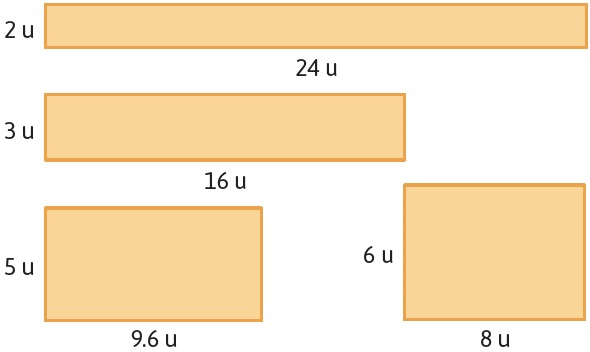
\includegraphics[width=0.9\textwidth]{ejem10.2}
          \caption{Grupo de rect\'angulos con medidas de largo y ancho para cada uno.}
          \label{fig:rectangulos}
        \end{figure}

        \begin{table}[!h]
          \centering
          \begin{tabular}{|l|c|c|c|}
            \hline
                         & Lado 1 (u) & Lado 2 (u) & Área (u$^2$) \\
            \hline
            Rectángulo 1 & 2          & 24         & 48           \\
            Rectángulo 2 & 3          &            &              \\
            Rectángulo 3 & 5          &            &              \\
            Rectángulo 4 & 6          &            &              \\
            \hline
          \end{tabular}
          \caption{}
          \label{tab:rectangulos}
        \end{table}
        \begin{enumerate}
          \item Completa la Tabla \ref{tab:rectangulos} que muestra la medida de los lados de un conjunto de rect\'angulos.
          \item ¿Cómo es la variación de los datos de la tabla? ¿Por qué?
          \item Si se añade el rectángulo cuyo lado 1 mide 4 u, ¿cuál es la medida del otro lado? ¿Cuál es su área? Expliquen su procedimiento.
          \item ¿Cómo es el área de los rectángulos?
        \end{enumerate}
\end{enumerate}



\subsection{Problemas sobre proporcionalidad directa e inversa}

Presentamos diversas situaciones que involucran la interpretación de relaciones directas e inversas.
Intenta resolver por tu cuenta cada situación. Luego, una vez que agotes todas tus estrategias, analiza con detenimiento las propuesta de resolución de cada situación.

\subsubsection{Ejemplos}
\include*{Ejemplos/ejemplo2.1.1}
\include*{Ejemplos/ejemplo2.1.2}
\include*{Ejemplos/ejemplo2.1.3}
\include*{Ejemplos/ejemplo2.1.4}
\newpage
\subsubsection{Ejercicios}
Copia en tu libreta las siguientes situaciones. Realiza, para cada uno de ellas, todas las operaciones y
procedimientos necesarios para obtener la respuesta a cada una de las preguntas. Al terminar, señala la
opción que contenga la respuesta correcta.
\begin{enumerate}%[start=1]%<--- start option fixes number for first item
  \item Un grupo de 20 obreros puede terminar una
        construcción en 40 días. Al cabo de 10 días de trabajo,
        se les unen obreros de otro grupo, de modo que en 15 días
        más terminan la obra.\\
        \textbf{¿Cuántos obreros había en el segundo grupo?}\\
        \emph{Escoge 1 respuesta:}\\
        \begin{hoptions}
          \item 20 obreros
          \item 5 obreros
          \item 10 obreros
          \item 15 obreros
        \end{hoptions}

  \item Mateo va en auto de su casa a la universidad. Si va a una velocidad promedio de 60 kilómetros por hora, tarda 1 hora.\\
        \textbf{¿Cuánto tiempo tardaría si fuera a 40 kilómetros por hora?}\\
        \emph{Escoge 1 respuesta:}\\
        \begin{hoptions}
          \item 1 hora y 30 minutos
          \item 30 minutos
          \item 1 hora y 20 minutos
          \item 2 horas
        \end{hoptions}

  \item En una tienda, se venden rollos de papel higiénico. Cada rollo cuesta 2 dólares, pero hay la siguiente oferta:
        Lleva 3 rollos de papel higiénico y paga s\'olo 2.
        María va a la tienda a comprar 20 rollos de papel higiénico en oferta.\\
        \textbf{¿Cuánto pagará por la compra?}\\
        \emph{Escoge 1 respuesta:}\\
        \begin{hoptions}
          \item 28 dólares
          \item 17 dólares
          \item 30 dólares
          \item 14 dólares
        \end{hoptions}

  \item Un grupo de 32 tejedores puede terminar un pedido de ponchos en 15 días. Al cabo de 5 días de trabajo, se les unen tejedores de otro grupo, de modo que en 8 días más terminan el pedido.\\
        \textbf{¿Cuántos tejedores había en el segundo grupo?}\\
        \emph{Escoge 1 respuesta:}\\
        \begin{hoptions}
          \item 8 tejedores
          \item 16 tejedores
          \item 32 tejedores
          \item 10 tejedores
        \end{hoptions}

  \item \textbf{¿Cuál ecuación muestra variación directa?}\\
        \emph{Escoge 1 respuesta:}\\
        \begin{hoptions}
          \item $\dfrac{1}{5}\cdot a=\dfrac{1}{b}$
          \item $a\cdot b=\dfrac{1}{5}$
          \item $a=5\cdot \dfrac{1}{b}$
          \item $\dfrac{a}{b}=5$
          \item $a\cdot b=5$
        \end{hoptions}

  \item \textbf{¿Cuál ecuación muestra variación inversa?}\\
        \emph{Escoge 1 respuesta:}\\
        \begin{hoptions}
          \item $2\cdot \dfrac{1}{a}=\dfrac{1}{b}$
          \item $\dfrac{1}{2}\cdot \dfrac{1}{a}=\dfrac{1}{b}$
          \item $2\cdot a=b$
          \item $\dfrac{a}{b}=\dfrac{1}{2}$
          \item $a\cdot b=2$
        \end{hoptions}

  \item En el mercado, 2 kilogramos de papa cuestan \$3.5 dólares.
        Sofía tiene \$25 dólares para comprar 14 kilogramos de papa.\\
        \textbf{¿Cuáles de las siguientes afirmaciones son correctas?}\\
        \emph{Elige todas las respuestas adecuadas:}\\
        \begin{hoptboxes}
          \item Deberá pagar \$7.5 dólares por 6 kilogramos de papa.\\
          \item Pagará \$14 dólares por 8 kilogramos de papa.\\
          \item Sofía recibirá \$0.50 dólares de vuelto.\\
          \item Sofía necesitará más dinero para realizar la compra.\\
        \end{hoptboxes}

\end{enumerate}

\newpage
\subsubsection{Problemas}

\begin{enumerate}
  \item Estás preparando limonada. La cantidad de azúcar que necesitas depende de la cantidad de limones que uses,
        como se muestra en la tabla \ref{tab:azucar_limon}.
        \begin{table}[!h]
          \centering
          \begin{tabular}{|l|c|c|c|}
            \hline
            Tazas de azúcar     & $\frac{1}{3}$ & 1 & 3 \\
            \hline
            Cantidad de limones & 1             & 3 & 9 \\
            \hline
          \end{tabular}
          \caption{}
          \label{tab:azucar_limon}
        \end{table}

        \textbf{¿Cuál es la constante de proporcionalidad entre las tazas de azúcar y los limones?}

  \item Un carpintero fabrica sillas, las cuales le cuestan \$250.00 elaborar cada una. Además, tiene costos fijos por la renta del local y equipo que es de \$3 500.00 al mes. \\
        \textbf{¿Cuántas sillas hacen que el precio por producirlas sea igual a los costos fijos?}\\

  \item El equipo conformado por Cristina, Javier y Claudia tardó 8 días en responder 120 preguntas que su profesor de Historia de México les dejó de tarea.
        \begin{enumerate}
          \item ¿Cuántas preguntas resolvieron Cristina, Javier y Claudia cada día?
                \begin{hoptions}
                  \item 3 preguntas \item 5 preguntas \item 8 preguntas \item 15 preguntas
                \end{hoptions}
          \item ¿Cuántas preguntas respondió cada uno de los integrantes del equipo por día?
                \begin{hoptions}
                  \item 3 preguntas \item 5 preguntas \item 8 preguntas \item 15 preguntas
                \end{hoptions}
          \item Si el equipo estuviera formado por 5 personas, ¿cuántas preguntas respondería cada una en un solo día, suponiendo que trabajan al mismo ritmo?
                \begin{hoptions}
                  \item 3 preguntas \item 5 preguntas \item 8 preguntas \item 15 preguntas
                \end{hoptions}
          \item ¿En cuántos días responderían las 120 preguntas si el equipo estuviera formado por 8 personas, suponiendo que trabajan al mismo ritmo que el equipo original?
                \begin{hoptions}
                  \item 3 días \item 5 días \item 8 días \item 15 días
                \end{hoptions}
          \item Si sólo hubieran sido 45 preguntas y el equipo estuviera formado por 5 personas que trabajan al mismo ritmo, ¿en cuantos días terminarían la tarea?
                \begin{hoptions}
                  \item 2 días \item 5 días \item 8 días \item 15 días
                \end{hoptions}
        \end{enumerate}

  \item Tania tiene 5 parejas de canarios y necesita 15 paquetes de comida para alimentarlos durante 30 días.
        \begin{enumerate}
          \item ¿Cuántos días podría alimentar a los canarios con un paquete de comida?\\
                \begin{hoptions}
                  \item  5 días
                  \item 10 días
                  \item 30 días
                  \item 90 días
                \end{hoptions}
          \item ¿Cuántos días podría alimentar a los canarios con el triple de alimento?\\
                \begin{hoptions}
                  \item 1 día
                  \item 2 días
                  \item 3 días
                  \item 5 días
                \end{hoptions}
          \item ¿Cuántos días le durarían los 15 paquetes de comida para alimentar al triple de canarios?\\
                \begin{hoptions}
                  \item 15 días
                  \item 30 días
                  \item 60 días
                  \item 90 días
                \end{hoptions}
          \item Si Tania tuviera un total de 10 parejas de canarios, ¿cuántos días podría alimentarlos con un
                solo paquete de comida?\\
                \begin{hoptions}
                  \item 5 días
                  \item 10 días
                  \item 30 días
                  \item 90 días
                \end{hoptions}
          \item Si Tania tuviera 30 canarios, ¿cuántos días le durarían 5 paquetes de comida?\\
                \begin{hoptions}
                  \item  1 día
                  \item 2 días
                  \item 3 días
                  \item 5 días
                \end{hoptions}
        \end{enumerate}
\end{enumerate}
\section{Reparto Proporcional}
Con lo que hemos aprendido sobre las proporciones directas e inversas, ahora trabajaremos en dividir cantidades de tal
manera que se usen estas variaciones.

\subsection{Situaciones de reparto proporcional}
\begin{mybox}{0.45\linewidth}{
    \begin{comfortaa}
      \color{white}Definici\'on
    \end{comfortaa}}
  \begin{minipage}{0.90\linewidth}
    Resolver un problema de reparto proporcional consiste en dividir una cantidad en partes que guarden entre sí
    ciertas razones. Para realizar el reparto, se encuentran los valores faltantes en una relación proporcional directa.
  \end{minipage}%
\end{mybox}
\subsubsection{Reparto proporcional directo}
\emph{A una mayor cantidad corresponde mayor proporción}

\begin{enumerate}
  \item Antonio y Laura vieron un anuncio para limpiar un jardín de 40 m$^2$ por una paga de \$800.
        \begin{enumerate}
          \item \textbf{¿Cuáles son las variables que se deben considerar para realizar el trabajo?}
                \begin{enumerate}
                  \item[\color{colorrds}\Large$\square$] Cantidad a pagar por el trabajo
                  \item[\color{colorrds}\Large$\square$] Cantidad de trabajadores
                  \item[\color{colorrds}\Large$\square$] Días a trabajar
                  \item[\color{colorrds}\Large$\square$] Superficie a limpiar
                  \item[\color{colorrds}\Large$\square$] Tipo de trabajo
                \end{enumerate}

          \item Si Antonio y Laura trabajaron el lunes y limpiaron la cuarta parte del jardín, \textbf{¿Qué cantidad les faltó por limpiar?}\\
                \begin{hoptboxes}
                  \item  5 m$^2$
                  \item 10 m$^2$
                  \item 30 m$^2$
                  \item 40 m$^2$
                  \item 50 m$^2$
                \end{hoptboxes}

          \item El martes fueron ayudados por sus dos primos. Manteniendo el mismo ritmo de trabajo que el lunes, \textbf{¿qué cantidad limpiaron el segundo día?}\\
                \begin{hoptboxes}
                  \item 10 m$^2$
                  \item 20 m$^2$
                  \item 30 m$^2$
                  \item 40 m$^2$
                  \item 50 m$^2$
                \end{hoptboxes}
          \item Laura y sus dos primos salieron de vacaciones por lo que Antonio terminará el trabajo. Toño está desanimado así que decide dividir el trabajo que resta en 4 días. \textbf{¿Qué superficie limpiará cada día?}\\
                \begin{hoptboxes}
                  \item 1 m$^2$
                  \item 2 m$^2$
                  \item 2.5 m$^2$
                  \item 3 m$^2$
                  \item 3.5 m$^2$
                \end{hoptboxes}
          \item De haber mantenido el ritmo de trabajo, \textbf{¿cuántos días le habría tomado a Antonio terminar el trabajo?}
                \begin{hoptboxes}
                  \item 1 d\'a
                  \item 2 d\'as
                  \item 3 d\'as
                  \item 4 d\'as
                  \item 5 d\'as
                \end{hoptboxes}
        \end{enumerate}
  \item Hay una oferta en la que se vende un lote de 126 canicas de colección a un precio de \$689 pesos.
        Pedro y Juan lo quieren comprar pero ninguno tiene suficiente dinero, así que Pedro le propone a Juan
        comprar el lote entre los dos y luego repartirse las canicas. Pedro coopera con \$449 y Juan completa el resto.

        \begin{enumerate}
          \item ¿Qué parte del total del precio puso Pedro?
          \item Si se considera que el reparto se haga de la misma manera, ¿qué parte del total de las canicas le corresponden a Pedro?
          \item ¿Cuántas canicas le corresponden a Pedro y cuántas a Juan?
          \item ¿Piensas que este reparto ha sido justo? ¿Por qué?
          \item ¿En qué sentido el reparto fue proporcional?
          \item ¿En qué tipo de proporción se basa esta manera de repartir? Explica.
        \end{enumerate}



  \item Para el Sorteo Gordo de Navidad de la Lotería Nacional, el cual repartirá un premio de \$397,952,000.00, tres amigos
        cooperan para comprar una serie completa de billetes de lotería (20 cachitos), como los de la figura \ref{fig:cachito}, que cuesta
        \$2,000.00, pues ninguno tiene esa cantidad de dinero. Antonio pone \$520.00, Beatriz coopera con \$680.00 y Carlos
        con \$800.00. Los tres amigos siguen la plática acerca de lo qué harán al ganarse el premio.
        \begin{figure}[H]
          \centering
          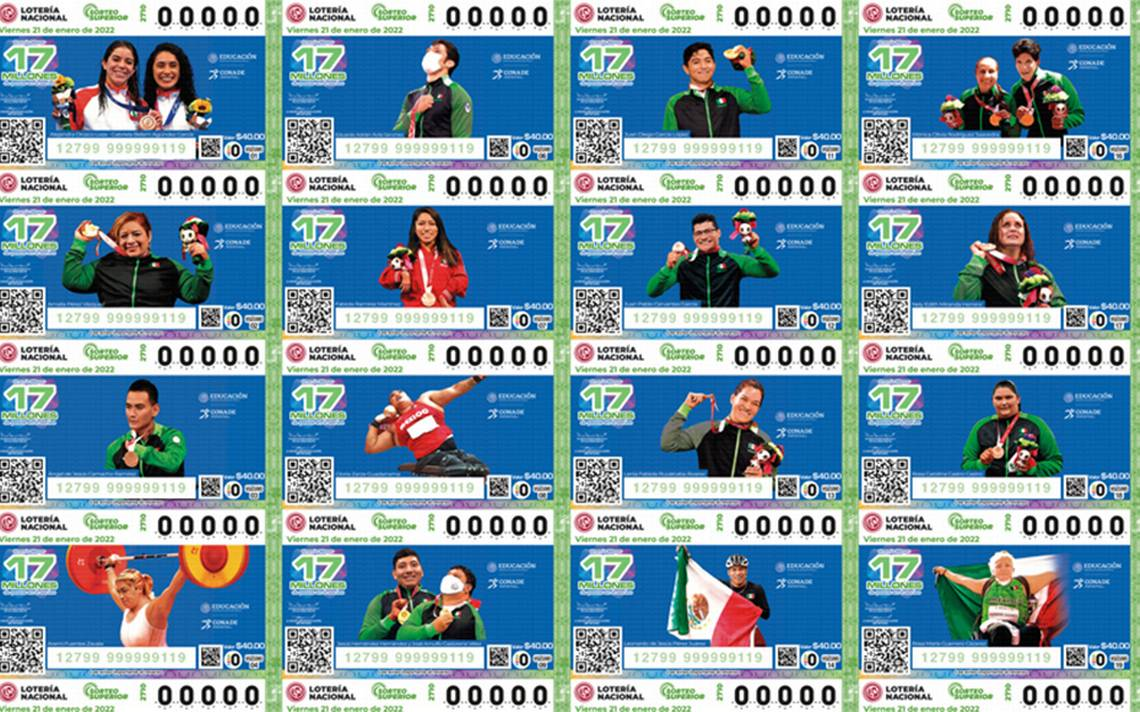
\includegraphics[width=0.4\textwidth]{cachito}
          \captionof{table}{Ilustración de una serie de la Loter\'ia Nacional.}
          \label{fig:cachito}
        \end{figure}
        \begin{enumerate}
          \item Carlos propone dividir el premio entre tres. Sin embargo, los otros dos amigos protestan diciendo que eso no es justo. ¿Cuánto dinero le tocaría a cada uno? Expliquen si es justo o no.
          \item Beatriz propone que cada quien tome el número de billetes de lotería que representa el dinero que invirtió y que cada quien cobre su premio. ¿Este reparto es proporcional? ¿Por qué? Usen trocitos de papel para comprobarlo.
          \item Completa la tabla \ref{tab:reparto_billetes} para calcular el reparto de billetes de lotería. ¿Se puede repartir de esta manera? ¿Por qué?
                \begin{figure}[H]
                  \centering
                  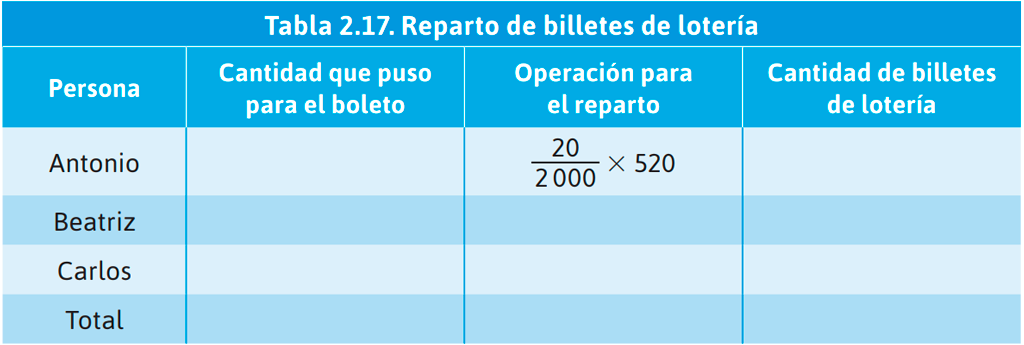
\includegraphics[width=0.7\textwidth]{tabla2.17.png}
                  \captionof{table}{Reparto de billetes de loter\'ia}
                  \label{tab:reparto_billetes}
                \end{figure}
          \item Antonio propone repartir el dinero del premio de manera proporcional a lo que cada uno invirtió. Completa la tabla \ref{tab:reparto_dinero} para calcular la cantidad de dinero que le corresponde a cada amigo.
                \begin{figure}[H]
                  \centering
                  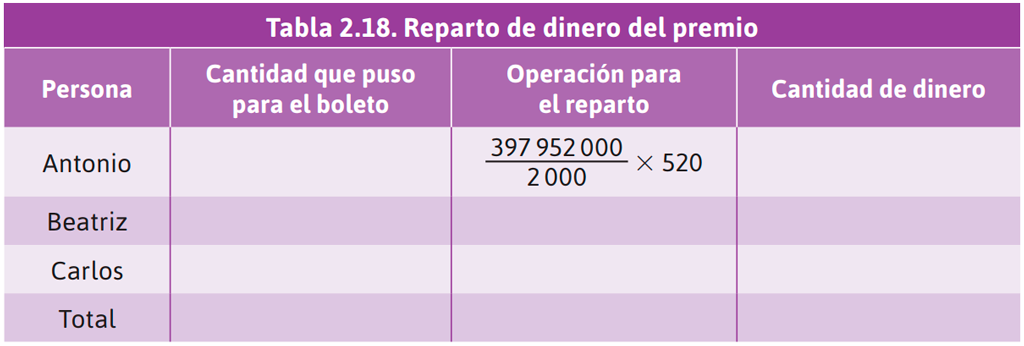
\includegraphics[width=0.7\textwidth]{tabla2.18.png}
                  \captionof{table}{Reparto de dinero del premio}
                  \label{tab:reparto_dinero}
                \end{figure}
          \item ¿Este reparto es proporcional? ¿Por qué?
          \item ¿Consideran justo este reparto? Explica.
          \item ¿Cómo se relaciona este reparto con una situación de proporcionalidad?
          \item ¿Hay una constante de proporcionalidad? Si es así, ¿cuál es?
          \item Propongan un procedimiento para hacer un reparto de manera proporcional.
          \item En grupo, planteen situaciones en las que un reparto proporcional resuelve satisfactoriamente un problema.
        \end{enumerate}
\end{enumerate}
\subsubsection{Reparto proporcional inverso}
En un problema de reparto proporcional inverso, se busca convertirlo en una proporción directa. Por ello, se utiliza el inverso multiplicativo o recíproco.
De manera adicional, en algunos casos se reparten las cantidades de tal manera que al menor le toque la mayor parte y viceversa.
\begin{enumerate}
  \item Un padre de familia tiene 3 hijos: Lucía, de 8 años; Julio, de 12, y Liliana, de 5 años. Repartirá entre ellos \$2 000.00 que ha ahorrado, de manera proporcional a sus edades, de tal manera que al hijo menor le toque la mayor parte del dinero.
        \begin{enumerate}
          \item Si aplican los procedimientos realizados en las actividades anteriores, ¿se cumple la condición que desea el padre? Expliquen.
          \item Completen la tabla \ref{tab:reparto_hijos} para calcular cuánto recibirá cada hijo.
                \begin{figure}[H]
                  \centering
                  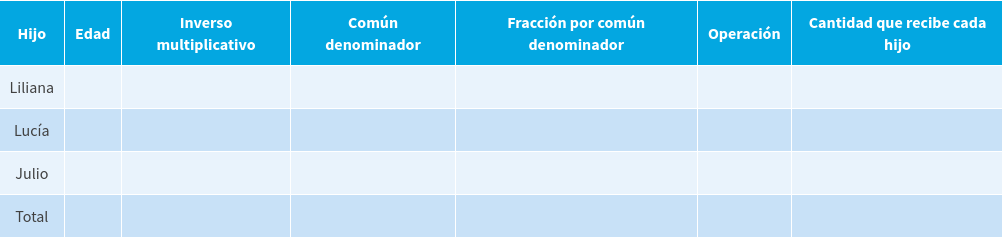
\includegraphics[width=\textwidth]{reparto_hijos}
                  \captionof{table}{Reparto de un padre de familia a sus tres hijos}
                  \label{tab:reparto_hijos}
                \end{figure}
          \item ¿Se cumple de esta manera el objetivo del padre de familia? ¿Por qué?
        \end{enumerate}

  \item Se repartirán \$2 200.00 en premios a los tres primeros lugares de una carrera de automóviles, de tal manera que el primer lugar reciba la mayor parte del monto.
        \begin{enumerate}
          \item ¿Qué tipo de reparto proporcional deben realizar? ¿Por qué?
          \item  Completen la tabla \ref{tab:reparto_carrera} para calcular los montos.
                \begin{figure}[H]
                  \centering
                  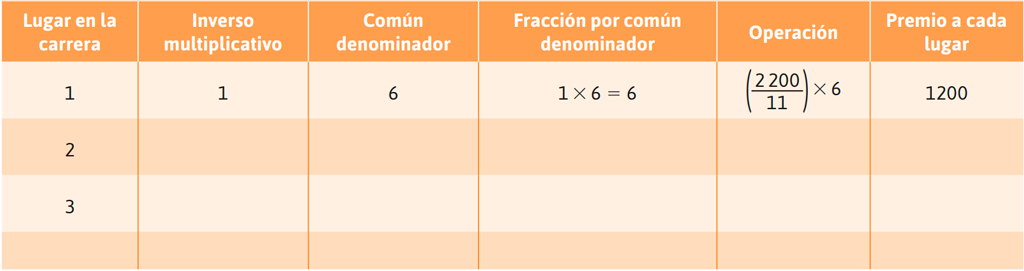
\includegraphics[width=\textwidth]{reparto_carrera}
                  \captionof{table}{Premio a los primeros 3 lugares}
                  \label{tab:reparto_carrera}
                \end{figure}
          \item ¿Se cumple el objetivo de la repartición de los premios? ¿Por qué?
          \item ¿Qué distingue a un problema de reparto proporcional inverso de uno directo?
          \item Describe un procedimiento para resolver un problema de reparto proporcional inverso.
        \end{enumerate}

\end{enumerate}


% \section{Sistemas de ecuaciones lineales con dos inc\'ognitas}
% \subsection{Ecuaciones lineales}
% \subsection{Sistemas de ecuaciones lineales con dos inc\'ognitas}

% \section{M\'etodos algebraicos de soluci\'on de sistemas de ecuaciones}
% \subsection{Soluci\'on de sistemas de ecuaciones}
% \subsection{Problemas sobre sistemas de ecuaciones lineales}
\newpage
\section{Variabilidad lineal y proporcionalidad inversa}
\subsection{Situiaciones de variación lineal}
Repasaremos las \textbf{características} principales de las variaciones lineales, a fin de tenerlas presentes al
compararlas con otras, como las de proporcionalidad inversa. Lee la situación, observa la imagen y responde lo que se pide.
\begin{enumerate}
  \item La balanza de resorte o dinamómetro es un dispositivo que mide el peso de un objeto.
        El funcionamiento consiste en la medición de la elongación de un resorte mediante una corredera
        móvil sobre una escala graduada. Supón que fijas un dinamómetro en el techo y colocas un peso
        de 10 kg. Luego, mides la elongación del resorte que es de 12 cm.\\
        \begin{minipage}[t]{0.15\linewidth}
          \begin{figure}[H]
            \centering
            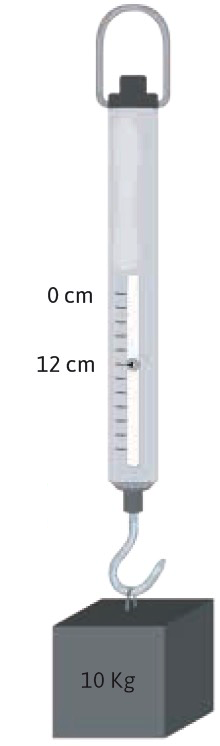
\includegraphics[width=\linewidth]{dinamometro}
            %\captionof{table}{Premio a los primeros 3 lugares}
            \label{fig:dinamometro}
          \end{figure}%
        \end{minipage}%
        \begin{minipage}[t]{0.85\linewidth}
          \begin{enumerate}
            \item ¿Cuánto se estira el resorte con un peso de 14 kg? Si éste se estiró 3 cm, ¿cuánto peso se colocó en él?
            \item ¿Qué tipo de variación se da entre el peso colocado al resorte y su estiramiento?
            \item ¿Cuál es la constante de proporcionalidad en esta relación?
            \item ¿Qué maneras tienes para representar esta variación? Realiza dichas representaciones.
            \item ¿Qué información es relevante para responder y cuál no?
            \item Describe los procedimientos desarrollados para identificar y representar la variación.
          \end{enumerate}

        \end{minipage}
        \newpage

        \begin{minipage}[t]{0.45\linewidth}
          \item En algunas ciudades, el servicio de taxi lo prestan compañías que cobran de manera distinta. Hay empresas que
          cobran una cantidad fija inicial, lo que se conoce como \emph{"banderazo"}, y luego otra cantidad por la distancia
          recorrida, sea por kilómetro o fracción de éste. Una ciudad cuenta con tres compañías de servicio de taxi:\\
          \begin{itemize}
            \item \emph{La cotorra}, que cobra \$13.50 el banderazo y \$3.50 por kilómetro.
            \item \emph{El volador}, que usa la expresión $c = 3d + 16$ para su tarifa, donde $c$ es el costo en pesos y $d$
                  el número de kilómetros recorridos.
            \item \emph{El acompañante}, que cobra \$4.00 por kilómetro sin banderazo.
          \end{itemize}
        \end{minipage}\hfill
        \begin{minipage}[t]{0.5\linewidth}
          \begin{figure}[H]
            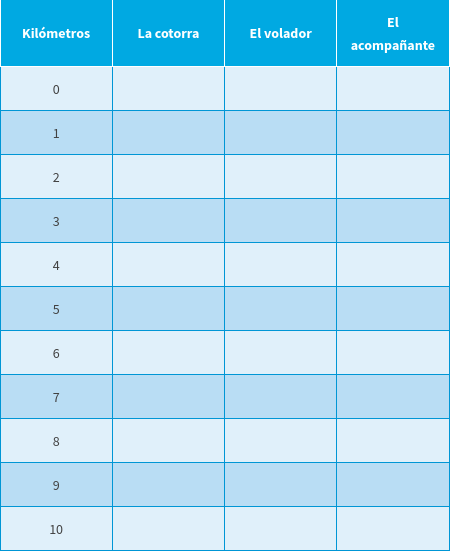
\includegraphics[width=\linewidth]{taxi}
            \captionof{table}{Costos por kilómetro (comparativo).}
            \label{fig:taxi}
          \end{figure}
        \end{minipage}

        \begin{enumerate}
          %\begin{minipage}[t]{\linewidth}
          \item Completa la tabla \ref{fig:taxi} para hacer un comparativo por kilómetro de las tres compañías.
          \item ¿Con qué compañía te conviene hacer un viaje de 3.5 km? ¿Por qué?
          \item ¿Con cuál es más económico un recorrido de 11$\frac{3}{4}$km? ¿Por qué?
          \item ¿Cuántos kilómetros recorres con \$50.00 en cada compañía? Describe en tu cuaderno los procedimientos
                para obtener estas cantidades:
                \begin{itemize}
                  \item La cotorra:
                  \item El volador:
                  \item El acompañante:
                \end{itemize}
          \item ¿Cómo varían, en cada caso, los costos por kilómetro de cada compañía?
          \item ¿Cuál costo por kilómetro varía más rápido?
                %\end{minipage}

          \item ¿Cuál varía más lento? De acuerdo con el contexto del problema, ¿es conveniente
                incluir valores negativos?
          \item ¿De qué tipo es la variación de los cobros en las tres compañías? Explica.
          \item ¿Cuánto se paga por un recorrido de 2 km en cada compañía?
          \item ¿Y cuánto por un recorrido de 4 km?
          \item ¿Cuál compañía cobra el doble si se recorren el doble de kilómetros?
          \item ¿Qué compañía cobra mediante una relación proporcional directa?
          \item ¿Cómo se identifica a partir de los valores de la tabla? Explica.
          \item ¿Cómo se determina la razón de cambio de cada compañía?
          \item ¿Qué relación existe entre la razón de cambio y la pendiente de una recta?
          \item ¿Qué significa que las compañías \emph{La cotorra} y \emph{El volador} cobren una cantidad de dinero aún sin
                haber recorrido ninguna distancia?
          \item ¿Cómo se relaciona este cobro con la ordenada al origen?
          \item Escribe una ecuación que represente los cobros de cada compañía:
                \begin{itemize}
                  \item La cotorra:
                  \item El volador:
                  \item El acompañante:
                \end{itemize}
          \item ¿Cómo construyes estas expresiones algebraicas?
          \item ¿Qué características tiene la representación tabular de una variación lineal?
          \item ¿Qué características tiene su expresión algebraica?
          \item Haz la gráfica de la figura \ref{fig:cartesian_taxi} que representa los cobros de las tres compañías de transporte. Luego resuelve lo que se te pide.
                \begin{figure}[H]
                  \centering
                  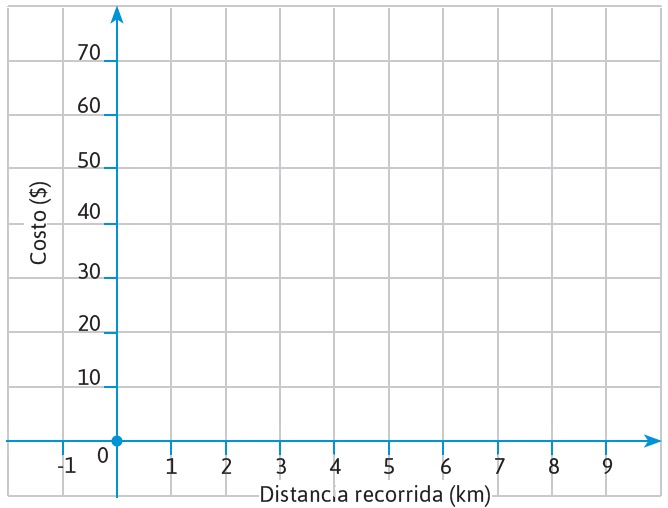
\includegraphics[width=0.5\linewidth]{cartesian_taxi}
                  \captionof{figure}{Gr\'afica de los costos por unidad de distancia recorrida de las tres compañ\'ias del corporativo.}
                  \label{fig:cartesian_taxi}
                \end{figure}%
                \begin{enumerate}
                  \item ¿Cuál es el valor de la razón de cambio para la representación del cobro de cada compañía? ¿Cómo determinaste estos valores?
                  \item ¿Cuál es el valor de la ordenada al origen en cada caso? Explica cómo lo obtuviste.
                  \item ¿Las gráficas crecen o decrecen? Explica.
                  \item ¿Qué características tiene la gráfica de una variación lineal?
                \end{enumerate}
        \end{enumerate}

        \newpage
  \item Un batitermógrafo es un aparato que se encuentra en los submarinos y que mide la temperatura del
        agua en sus profundidades. La tabla \ref{tab:table_bati} muestra la temperatura registrada por dicho aparato cada 200 metros
        de profundidad en un cierto lugar del océano.\\
        \begin{minipage}[t]{0.35\linewidth}
          \begin{figure}[H]
            \centering
            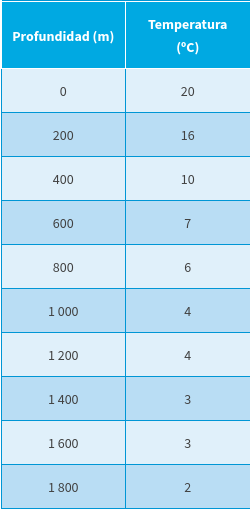
\includegraphics[width=\linewidth]{table_bati.jpg}
            \captionof{table}{Tabla de la temperatura del agua en cada profundidad de medición.}
            \label{tab:table_bati}
          \end{figure}%
        \end{minipage}\hfill
        \begin{minipage}[t]{0.6\linewidth}
          \begin{figure}[H]
            \centering
            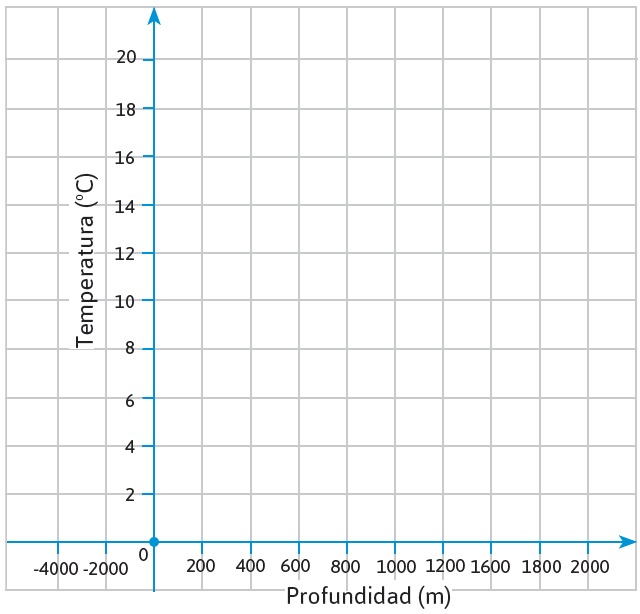
\includegraphics[width=\linewidth]{cartesian_bati.jpg}
            \captionof{figure}{Gr\'afica de la temperatura del agua en cada profundidad de medición.}
            \label{fig:cartesian_bati}
          \end{figure}
        \end{minipage}
        \begin{enumerate}
          \item ¿Cuántos grados desciende la temperatura entre los 400 m y los 1,800 m de profundidad?
          \item ¿Cuántos grados baja la temperatura entre los 1,000 m y los 1,200 m?
          \item ¿Es una tabla que representa una variación lineal? Explica por qué.
          \item ¿Qué características de una tabla que representa una variación lineal no se tienen en este problema?
          \item Traza la gráfica en la figura \ref{fig:cartesian_bati} que modele la temperatura de acuerdo con la profundidad.
          \item Indiquen los intervalos en los que la temperatura se mantiene constante al descender el submarino.
          \item ¿Hay intervalos donde la gráfica es creciente? ¿Por qué?
          \item ¿Cuál es la razón de cambio en esta variación? Explica.
          \item ¿Qué características de la gráfica de una variación lineal no se presentan en esta situación?
          \item ¿Cómo describes la variación de la temperatura respecto a los metros que se descienden?
        \end{enumerate}
  \item Un paralelogramo tiene las medidas indicadas en la figura \ref{fig:paralelogramo_fig}.
        Para que el área se mantenga constante, ¿cuánto debe medir la base si la altura aumenta 3 cm?

        \begin{minipage}[t]{0.35\linewidth}
          \begin{figure}[H]
            \centering
            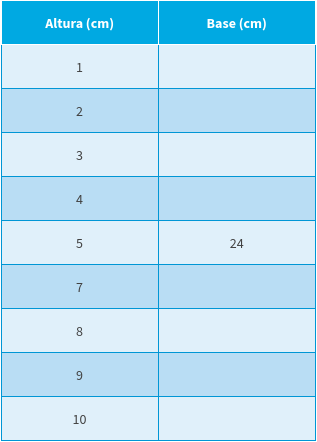
\includegraphics[width=\linewidth]{paralelogramo.png}
            \captionof{table}{Tabla con las medidas de Base y Altura del paralelogramo de la figura \ref{fig:paralelogramo_fig}.}
            \label{tab:paralelogramo_table}
          \end{figure}%
          \begin{figure}[H]
            \centering
            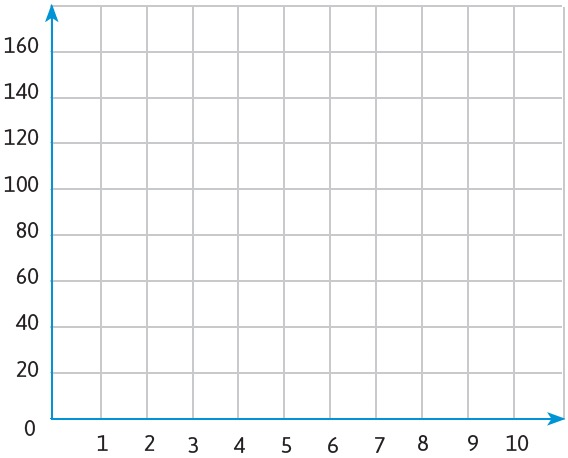
\includegraphics[width=\linewidth]{cartesian_blank}
          \end{figure}
        \end{minipage}\hfill
        \begin{minipage}[t]{0.65\linewidth}
          \begin{figure}[H]
            \centering
            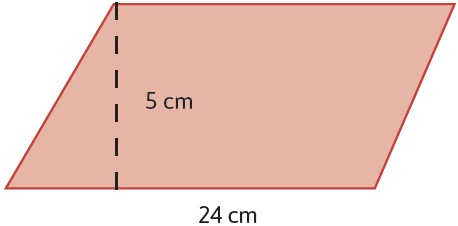
\includegraphics[width=0.7\linewidth]{paralelogramo.jpg}
            \captionof{figure}{Figura geom\'etrica paralelogramo}
            \label{fig:paralelogramo_fig}
          \end{figure}
          \begin{enumerate}
            \item ¿Qué operaciones realizan para conocer la medida de la base con este cambio en la altura?
            \item ¿Cuál es el valor de la base?
            \item ¿Qué tipo de relación proporcional se da entre la base y la altura si el área se mantiene constante? Explica.
            \item De acuerdo con las operaciones para este caso, completen la tabla \ref{tab:paralelogramo_table} calculando las medidas de la base
                  dadas las de la altura.
            \item ¿Qué operaciones realizaron para saber cada medida de la base del paralelogramo al variar la altura?
            \item Describan un procedimiento para obtener el valor de la base (y), dado cualquier valor de la altura (x)
                  y manteniendo constante el área:
            \item Escriban una expresión algebraica que describa el procedimiento que han desarrollado.
            \item Construyan una gráfica que muestre la variación de la base y la altura de la actividad anterior.
            \item ¿Qué características tiene esta gráfica?
            \item ¿Se puede obtener el valor de la razón de cambio? ¿Es posible saber el valor de la ordenada al origen? Expliquen.
            \item ¿Esta gráfica es creciente o decreciente? ¿Por qué?
            \item ¿Qué sucede si $x = 0$ en la expresión algebraica? ¿Cómo se observa este hecho en la gráfica?
            \item ¿Qué sucede si la altura es igual a 0? ¿Es posible esto en la situación planteada? ¿Por qué?
          \end{enumerate}
        \end{minipage}
\end{enumerate}
\newpage
\subsubsection{Ejercicios}
\begin{enumerate}

  \item Luisa trabaja en una tienda de artículos deportivos. Tiene un sueldo mensual de \$4 500 y recibe una comisión
        de \$50 por cada artículo que vende.
        \begin{enumerate}
          \item ¿Cuánto dinero recibiría Luisa si vende 18 artículos en un mes?
          \item  ¿Cuántos obtendría si vende 37 artículos en el mismo lapso?
          \item  ¿Cuántos artículos tendría que vender Luisa al mes para ganar \$7,000?
          \item Si Luisa ganara \$3 500 al mes y recibiera \$55 por cada artículo vendido,
                ¿con qué expresión podría representarse esta situación?
          \item Escribe una expresión que permita conocer cuánto gana Luisa al mes.
        \end{enumerate}
  \item En una carrera automovilística uno de los pilotos inició 30 m antes de la línea de salida con una rapidez constante de 145 km/h.
        \begin{enumerate}
          \item ¿Qué distancia, a partir de la línea de salida, habría recorrido el automóvil después de 5 minutos?
          \item A partir de la línea de salida, ¿qué distancia recorrería el automóvil en 17 minutos?
          \item ¿En cuántos minutos recorrería 200 km?
          \item Escribe una expresión que permita conocer la distancia que recorrería el automóvil respecto al
                tiempo, si hubiese iniciado en la línea de salida.
          \item ¿Cuál sería la expresión que representa la situación original?
        \end{enumerate}

  \item En una competencia de caminata, un atleta ha recorrido 1.6 kilómetros en 8 minutos y mantiene ese mismo ritmo en todo el recorrido.
        \begin{enumerate}
          \item Representa de manera tabular, gráfica y algebraica la carrera del atleta cada 8 min durante 1 h.
          \item Si la caminata es de 50 kilómetros, ¿en qué tiempo termina la competencia?
        \end{enumerate}

\end{enumerate}
\newpage
\subsection{Representaciones de proporcionalidad inversa}
Anteriormente hemos trabajado con situaciones de proporcionalidad inversa, por lo que recordaremos cómo identificar
un problema con este tipo de proporción, así como sus características principales.\\

Lee la situación y responde lo que se pide.\\

\begin{enumerate}
  \item Para pintar una superficie determinada, el número de pintores que aparecen en la imagen tardan 80 horas,
        por lo que uno de ellos considera que hay que contratar más pintores para acabar antes con el trabajo.
        \begin{enumerate}
          \item ¿En cuánto tiempo lo harían 4 pintores más?
          \item Si al contrario, del grupo original renuncian 2, ¿en cuánto tiempo harían el trabajo los restantes?
          \item ¿Qué tipo de variación se da entre el número de pintores y los días que ocupan en su labor?
          \item ¿Cuál es la constante de proporcionalidad en esta relación?
          \item ¿Qué maneras tienes para representar esta variación? Realiza dichas representaciones.
          \item ¿Qué información es relevante para responder y cuál no?
          \item Describe los procedimientos realizados para identificar y representar la variación.
          \item Reúnanse en equipo. Expresen las características de una variación inversa cuando se representa con
                gráficas o expresiones algebraicas. Argumenten o corrijan sus resultados si es necesario.
        \end{enumerate}
  \item Verónica es costurera y le han encargado que haga banderas iguales a partir de una pieza de tela de 60 m de largo.
        \begin{enumerate}
          \item Si cada bandera se hiciera con 2 m de tela, ¿cuántas se pueden hacer con los 60 m?
          \item Y si fueran de 5 m de largo, ¿cuántas se podrían hacer?
          \item ¿Cuáles fueron tus operaciones para conocer estas cantidades?
          \item Si se le pidieron 50 banderas, ¿de cuántos metros sería cada una?
          \item Y si el pedido fue de 90, ¿cuáles serían sus medidas?
          \item ¿Qué operaciones realizaste en este caso?
          \item ¿Qué pasa con la medida de cada bandera si aumenta la cantidad de banderas que se tienen que hacer?
                ¿Y qué pasa si disminuye la cantidad de banderas? Si la cantidad de banderas que se tienen que hacer aumenta al doble,
                ¿cómo varían las medidas de dichas banderas?
          \item ¿Qué tipo de relación se da entre el número de banderas y la medida de cada una? Explica.
          \item Al multiplicar las medidas de cada bandera con su correspondiente cantidad de banderas que se pueden hacer,
                ¿qué cantidad se obtiene en cada caso? ¿Cómo se puede interpretar este resultado? ¿Qué significa esta cantidad?
          \item ¿Cuál es la constante de proporcionalidad?
        \end{enumerate}
  \item Martín ha pagado \$2 700.00 para asistir durante 30 días a un club deportivo. Sólo irá una vez al día pero
        lo hará diario, sin falta.\\
        \begin{minipage}[t]{0.35\linewidth}
          \begin{figure}[H]
            \centering
            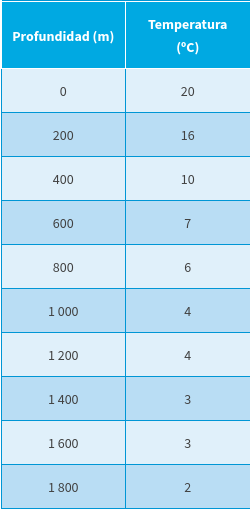
\includegraphics[width=\linewidth]{table_bati.jpg}
            \captionof{table}{Tabla de la temperatura del agua en cada profundidad de medición.}
            \label{tab:table_bati}
          \end{figure}%
        \end{minipage}%
        \begin{minipage}[t]{0.65\linewidth}
          \begin{enumerate}
            \item ¿Cuánto será el precio por día en el sexto día de asistir al club? ¿En qué día el precio por día será
                  de \$300.00?
            \item ¿Qué operaciones realizaste en cada caso?
            \item Completa la tabla 2.34. En tu cuaderno completa una similar pero con 30 días. Usa calculadora.
            \item ¿Qué parte representa el costo por día en el décimo día respecto al primer día de asistencia al club?
            \item ¿Qué tipo de variación se tiene entre el número de días en los que Martín visita el club y el precio
                  por día? Explica.
            \item ¿Cuál es la constante de proporcionalidad en este caso? ¿Cómo la determinas?
            \item ¿Qué características tiene una situación proporcional inversa? ¿Esta situación es una de este tipo?
            \item ¿De qué manera se distingue una tabla de una proporción inversa respecto a otro tipo de variaciones.
            \item Reúnanse en equipo con el propósito de recordar las características de una proporción inversa.
                  Corrijan o argumenten si consideran necesario.
          \end{enumerate}
        \end{minipage}
\end{enumerate}

\newpage
\subsubsection{Ejercicios}
\begin{enumerate}
  \item Lee el problema que se presenta y busca las cantidades en letras que se piden.
        Victor tiene una tira de madera de 400 cm de largo. Cortará la tira para tener palitos para banderas.
        \begin{figure}[H]
          \centering
          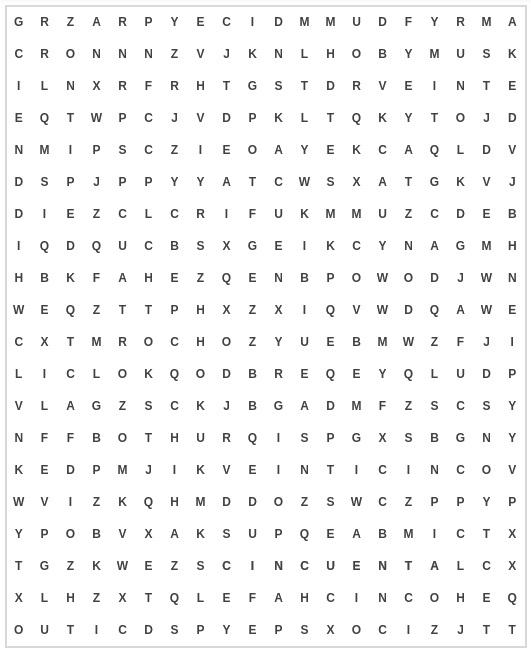
\includegraphics[width=0.75\linewidth]{sopa}
        \end{figure}%
        \begin{itemize}
          \item Longitud de cada palito, si en total corta 4.
          \item Longitud de cada palito, si en total corta 16.
          \item Longitud de cada palito, si en total corta 20.
          \item Cantidad de palitos, si cada uno mide 100 cm.
          \item Cantidad de palitos, si cada uno mide 80 cm.
          \item Cantidad de palitos si cada uno mide 50 cm.
          \item Cantidad de palitos, si cada uno mide 40 cm.
        \end{itemize}
        \newpage
  \item Escribe sobre la l\'inea de cada inciso, las palabras que completan las afirmaciones correctamente.
        Martha pagó \$3 000 por un curso de repostería y podrá asistir 30 días una hora diaria.
        Al realizar el pago le comentaron que no habría reembolso en caso de que no asistiera.

        \begin{enumerate}
          \item De acuerdo con los datos, cada día del curso costó \$\rule{2cm}{0.2pt}
          \item Martha enfermó y no pudo asistir los primeros 5 días, los \$3 000 que pagó corresponden a
                25 días, así cada día cuesta \$\rule{2cm}{0.2pt}
          \item Entre más días falte al curso, el costo de cada día \rule{2cm}{0.2pt}. (Se mantiene / disminuye / aumenta)
          \item Durante los días restantes Martha faltó \rule{2cm}{0.2pt} días más, por lo que cada día terminó costando \$150.
          \item Antes de inscribirse a este curso, Martha había visto otra opción en la que cada día costaba \$200.
                De hecho Martha pudo faltar \rule{2cm}{0.2pt} días más, y aún así, este curso resulta más barato.
        \end{enumerate}
\end{enumerate}

\newpage
\section{Modelos de variación lineal y proporcionalidad inversa}
Otras situaciones se pueden describir por medio de las variaciones proporcionales inversas. Veamos algunos casos y recordemos las propiedades de este tipo de variaciones.
\subsection{Modelos de variación lineal y proporcionalidad inversa}
\begin{enumerate}

  \item Lee la situación, observa la imagen de la figura \ref{fig:mapa} y responde lo que se pide.\\
        La familia Gómez se fue de día de vacaciones a Oaxtepec, que se encuentra a 100 km de distancia de donde viven. Cuando se dirigían al lugar, viajaron a una velocidad promedio de 80 km/h.
        De regreso había un poco de tránsito, por lo que recorrieron los 100 km de distancia en dos horas.
        \begin{figure}[H]
          \centering
          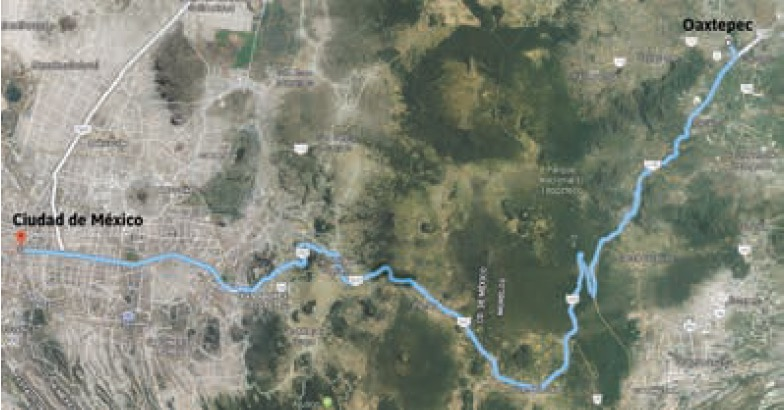
\includegraphics[width=0.75\linewidth]{mapa}
          \captionof{figure}{Ruta Ciudad de México - Oaxtepec.
            Fuente: http://edutics.mx/w7k. (Consulta: 20 de septiembre de 2018).}
          \label{fig:mapa}
        \end{figure}%
        \begin{enumerate}
          \item ¿Cuánto tiempo tardaron en el recorrido de ida?
          \item ¿A qué velocidad viajaron de regreso?
          \item ¿Qué tipo de variación se da entre la velocidad y el tiempo que tardaron en el viaje?
          \item ¿Cuál es la constante de proporcionalidad en esta relación?
          \item ¿Qué información es relevante para responder y cual no?
          \item Describe los procedimientos realizados para calcular los datos faltantes, así como para representar la variación.
        \end{enumerate}

        En situaciones que suceden en diferentes disciplinas, nos encontramos con que podemos modelarlas mediante una variación lineal.\\
        \newpage
  \item Analiza la situación y responde lo que se pide.\\

        Jaime estudia Medicina. En una clase ha aprendido que hay una nueva generación de fármacos en los que la cantidad de
        sustancia activa decae poco a poco hasta que el cuerpo la elimina completamente. Por ejemplo, un enfermo toma una
        medicina con 5 mg de sustancia activa, la cual decae 0.5 mg por día. Por lo que su profesor les solicita que describan
        la relación entre cantidad de sustancia activa y los días que dura dentro del cuerpo.

        \begin{figure}[H]
          \centering
          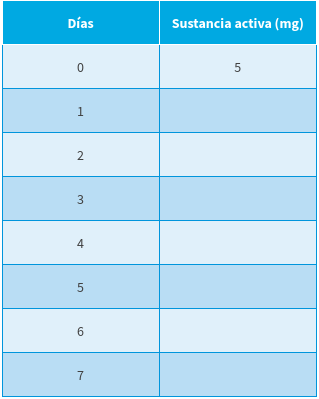
\includegraphics[width=0.75\linewidth]{farmacos}
          \captionof{table}{Tabla que relaciona la cantidad de sustancia activa de acuerdo con los d\'ias.}
          \label{tab:farmacos}
        \end{figure}%
        \begin{enumerate}
          \item Completa la tabla \ref{tab:farmacos} en la que se calcula diariamente la cantidad de sustancia activa dentro del enfermo.
          \item ¿Cómo cambia la cantidad de sustancia activa conforme pasan los días? ¿Puedes identificar un patrón en la disminución de la sustancia activa? ¿Cuál es?
          \item ¿Cómo se relaciona ese patrón con la constante de proporcionalidad?
          \item ¿Cuál es la razón de cambio? ¿Cómo se relaciona ésta con la constante de proporcionalidad? ¿Cuál es? Explica su obtención.
          \item Escribe una expresión algebraica que describa la situación.
          \item ¿En cuántos días la sustancia activa queda totalmente eliminada del organismo del enfermo? Explica.
          \item Traza la gráfica en la figura \ref{fig:farmacos_tabla} que describe la relación de la sustancia activa con los días que pasan.
                \begin{figure}[H]
                  \centering
                  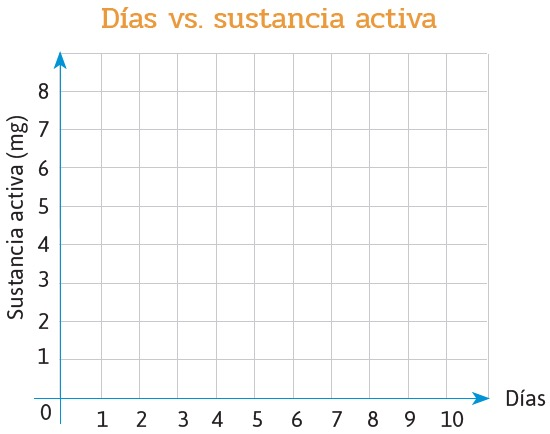
\includegraphics[width=0.75\linewidth]{farmacos_tabla}
                  \captionof{table}{Tabla que relaciona la cantidad de sustancia activa de acuerdo con los d\'ias.}
                  \label{fig:farmacos_tabla}
                \end{figure}%
          \item ¿La gráfica es ascendente o descendente? ¿Cómo se ve esto reflejado en la pendiente?
          \item ¿Cuál es el valor de la pendiente y de la ordenada al origen? Describe su obtención:
        \end{enumerate}

        \newpage
  \item Define la estrategia y procedimientos para responder a la siguiente situación.\\

        La gráfica de la figura \ref{fig:carro_control} muestra la relación entre el tiempo (t) que tarda un carro de control remoto en recorrer una distancia (d) fija de 50 m y la velocidad (v) que puede tener.
        \begin{minipage}[t]{0.45\linewidth}
          \begin{figure}[H]
            \centering
            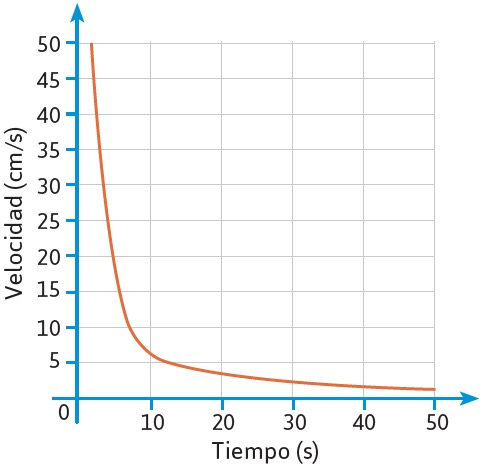
\includegraphics[width=\linewidth]{carro_control.jpg}
            \captionof{figure}{Gráfica correspondiente al movimiento del carrito de jugete.}
            \label{fig:carro_control}
          \end{figure}%
          \begin{figure}[H]
            \centering
            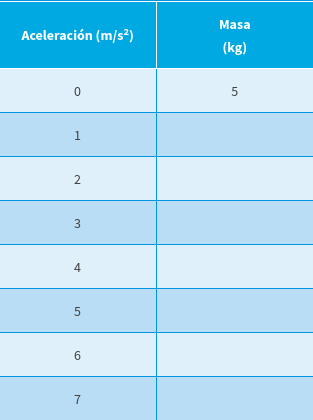
\includegraphics[width=\linewidth]{carro_control_tabla.jpg}
            \captionof{table}{Tabla correspondiente al movimiento del carrito de jugete.}
            \label{tab:carro_control_tabla}
          \end{figure}%
        \end{minipage}%
        \begin{minipage}[t]{0.5\linewidth}
          \begin{enumerate}
            \item De acuerdo con la gráfica, ¿cómo es la relación entre la velocidad y el tiempo? Explica.
            \item ¿Cuál es la constante de proporcionalidad para esta situación? Describe cómo la obtienen.
            \item ¿La gráfica crece o decrece? Explica.
            \item ¿En qué intervalos crece o decrece más rápido?
            \item ¿Y en cuáles crece o decrece más lento?
            \item ¿Qué sucede cuando $x$ se acerca a 0?
            \item ¿Se puede tener el caso $x = 0$? Explica.
            \item ¿Qué significa en la situación que $x=0$?
            \item ¿Qué sucede con la gráfica si los valores de $x$ aumentan?
            \item ¿Qué significa esto en la situación?
            \item Con los datos obtenidos de la gráfica, completa la tabla \ref{tab:carro_control_tabla}.
            \item ¿Qué operaciones realizan para obtener los datos de la tabla en cada caso?
            \item A partir de las operaciones que realizaron, escriban una expresión algebraica que describa la situación.
          \end{enumerate}
        \end{minipage}

  \item Analiza la situación y realiza lo que se les pide.\\

        La ley de la demanda indica que cuando el precio de un producto aumenta, la cantidad demandada disminuye;
        y cuando el precio del producto disminuye, la cantidad demandada aumenta. Supón que un impresor cobra \$3240.00
        por estampar una playera, por estampar 9, \$360.00 y por 90, diez veces menos.
        \begin{enumerate}
          \item ¿Cuál es la expresión que determina cuánto cobra el impresor? Explica cómo la determinaste.
          \item ¿Qué tipo de variación proporcional se tiene en la situación? Expliquen.
          \item ¿Cuál es el costo por estampar 20 playeras?
          \item ¿Cuántas playeras estampó el impresor si el precio fue de \$40.50?
          \item Describan sus procedimientos para obtener cada cantidad.
          \item Tracen en su cuaderno la gráfica que describe el precio por estampado con respecto al número de playeras.
          \item Con otros equipos, analicen las características de la gráfica y la expresión algebraica de una variación proporcional inversa. Argumenten sus respuestas y corrijan si es necesario.
        \end{enumerate}

        \boxabstract{Retoma la situación de la actividad de inicio y responde, completa o corrige tus respuestas. Reflexiona acerca de los conocimientos o habilidades que necesitabas al inicio y que ahora has adquirido. Escribe en tu cuaderno una conclusión.
          La masa de un material se puede obtener multiplicando la densidad de ese material por el volumen que ocupa. Un cuerpo de 3 kg/m3 de densidad ocupa un volumen de 0.8 m3, otro cuerpo con densidad de 5 kg/m3 tiene la misma masa que el anterior.
          Escribe la relación entre la densidad y el volumen para el segundo cuerpo.
          ¿Qué volumen tiene el segundo cuerpo?
          Realiza en tu cuaderno las representaciones tabular, gráfica y algebraica de esta situación.}
\end{enumerate}
\newpage
\subsubsection{Ejercicios}
\begin{enumerate}
  \item Analiza el caso de una medicina con una sustancia activa de 5 mg que decae 0.5 mg diario.
        \begin{enumerate}
          \item ¿Cómo es el tiempo que permanece en el cuerpo de un paciente, una sustancia activa
                de 5 mg que decae 0.5 mg cada dos días con relación al tiempo que permanece la sustancia activa inicial?\\
                \begin{hoptions}
                  \item Es la mitad
                  \item Es el mismo
                  \item Es el doble
                  \item No hay relación
                \end{hoptions}
          \item¿Cómo es el tiempo que permanece en el cuerpo de un paciente, una sustancia activa de 10 mg que decae
                1 mg diario con relación al tiempo que permanece la sustancia activa inicial?\\
                \begin{hoptions}
                  \item Es la mitad
                  \item Es el mismo
                  \item Es el doble
                  \item No hay relación
                \end{hoptions}
          \item ¿Cómo es el tiempo que permanece en el cuerpo de un paciente, una sustancia activa de 5 mg que decae 1 mg
                cada dos días con relación al tiempo que permanece la sustancia activa del inciso anterior?\\
                \begin{hoptions}
                  \item Es la mitad
                  \item Es el mismo
                  \item Es el doble
                  \item No hay relación
                \end{hoptions}
          \item ¿Cómo es la razón de cambio de una sustancia activa de 4 mg en el cuerpo humano que decae 1 mg diario con
                relación a la razón de cambio de la sustancia del inciso anterior?\\
                \begin{hoptions}
                  \item Es igual
                  \item Es mayor
                  \item Es menor
                  \item No hay relación
                \end{hoptions}
          \item ¿Cómo es la razón de cambio de una sustancia activa de 8 mg en el cuerpo humano que decae 1 mg cada dos
                días con relación a la razón de cambio de la sustancia del inciso anterior?\\
                \begin{hoptions}
                  \item Es igual
                  \item Es mayor
                  \item Es menor
                  \item No hay relación
                \end{hoptions}
        \end{enumerate}

  \item Ordena las sustancias de mayor a menor según el tiempo que permanecen en el cuerpo humano.

        \begin{hoptboxes}
          \item Sustancia de 5 mg que decae 0.5 mg diario.\\

          \item Sustancia de 8 mg que decae 1 mg diario.\\

          \item Sustancia de 3 mg que decae 1 mg cada dos días.\\

          \item Sustancia de 5 mg que decae 0.5 mg cada medio día.\\

          \item Sustancia de 6 mg que decae 0.5 mg diario.\\
        \end{hoptboxes}
\end{enumerate}

\newpage
\section{Per\'imetro y \'area de pol\'igonos regulares}
\subsection{Per\'imetro y \'area de pol\'igonos}

\section{\'Area del c\'irculo}


\subsection{Area del c\'irculo}
El área de un círculo es la cantidad de espacio que abarca. También podemos pensarla como la cantidad total de espacio dentro del círculo.
Para encontrar el área de un círculo podemos utilizar la siguiente fórmula:
\[A=\pi r^2\]

\subsubsection{Ejemplo 1: encontrar el área, dado el radio}
Encuentra el área de un círculo de radio 5.
\begin{figure}[H]
  \centering
  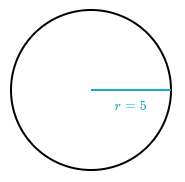
\includegraphics[width=0.5\textwidth]{./Unidad 2/Images/figS10_001.png}
\end{figure}
La ecuación para el área de un círculo es:
\begin{align*}
  A & = \pi r^2    \\
  A & = \pi 5^2    \\
  A & = \pi r^{25}
\end{align*}

Podemos detenernos aquí y escribir la respuesta como $25\pi$. O bien, podemos sustituir 3.14 por $\pi$ y multiplicar.\\
$A = 3.14 \cdot 25$\\
$A = 78.5$ unidades cuadradas\\
El área del círculo es $25\pi$ unidades cuadradas, o sea 78.5 unidades cuadradas.
\subsubsection{Ejemplo 2: encontrar el área, dado el diámetro}
Encuentra el área de un círculo de diámetro 16.
\begin{figure}[H]
  \centering
  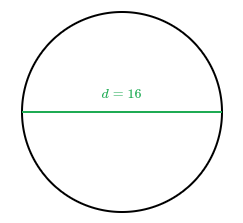
\includegraphics[width=0.5\textwidth]{./Unidad 2/Images/figS10_002.png}
\end{figure}
Primero encontremos el radio:

\begin{align*}
  r & = \dfrac d2     \\
  r & = \dfrac{16}{2} \\
  r & = 8
\end{align*}

Ahora podemos encontrar el área.\\

La ecuación para el área de un círculo es:
\begin{align*}
  A & = \pi r^2      \\
  A & = \pi \cdot 8  \\
  A & = \pi \cdot 64 \\
\end{align*}
Podemos detenernos aquí y escribir la respuesta como $64\pi$. O bien, podemos sustituir 3.14 por $\pi$ y multiplicar.\\
$A = 3.14 \cdot 64$\\
$A = 200.96$ unidades cuadradas\\

El área del círculo es $64\pi$ unidades cuadradas, o sea 200.96 unidades cuadradas.

\section{Medidas de tendencia central, rango y desviación media}
\subsection{Medidas de tendencia central}
\subsection{Rango y dispersi\'on de datos}
\subsection{Desviaci\'on media}


%%% U3
\chapter{}

\section{Sucesiones y equivalencia de expresiones}
\subsection{Reglas aritméticas y equivalencias}

\section{Figuras geométricas y equivalencia de expresiones}
\subsection{Equivalencia de expresiones algebraicas}
\subsection{Expresiones de perímetros y áreas}

\section{Volumen de prismas rectos}
\subsection{Volumen de primas rectos con base en forma de polígono regular}
\subsection{Problemas de volumen de prismas rectos}

\section{Volumen de cilindros rectos}
\subsection{Volumen de cilindros rectos}
\subsection{Problemas de cilindros rectos}

\section{Desarrollos planos de prismas y cilindros rectos}
\subsection{Desarrollos planos}

\section{Probabilidad teórica}
\subsection{Definición de probabilidad teórica}
\subsection{Probabilidad teórica y frecuencial}

\end{document}